\documentclass[a4paper]{article}

\usepackage{fullpage} % Package to use full page
\usepackage{parskip} % Package to tweak paragraph skipping
\usepackage{tikz} % Package for drawing
\usepackage{amssymb,amsmath,amsthm}
\usepackage{hyperref}
\graphicspath{ {../SP20/images/} }
\title{Automata and Numeration Systems}

\author{
Authors: Jack Gentile, Erik Joan Hernandez, Dun ``Eric" Ma, Stephen O'Brien, \\Haozhe ``Howard" Wang\\
Graduate Mentors: Eion Blanchard and Alexi Block Gorman\\
Faculty Advisors: Philipp Hieronymi and
Erik Walsberg\\
}
\date{December 21, 2018}

\newtheorem{definition}{Definition}
\newtheorem{theorem}{Theorem}

\begin{document}

\maketitle

\section{Introduction}

\subsection{Automata}

	\begin{definition}A \textbf{nondeterministic finite automaton}, or briefly an nfa, over alphabet $\Sigma$ is a quadruple $A = (S, I, T, F)$, where
	\begin{itemize}
		% \setlength{\itemsep}{-30pt}
		\item $S$ is a finite nonempty set called the set of \textbf{states}.\\
		\item $I$ is a subset of $S$ called the set of \textbf{initial states}.\\
		\item $T \subset S \times \Sigma \times S$ is a nonempty set called the \textbf{transition table} or \textbf{transition diagram}.\\
		\item $F$ is a subset of $S$ called the set of \textbf{final states}.
	\end{itemize}
\end{definition}

\begin{definition}
A \textbf{run} of A is a sequence $s_1...s_{n+1}$ on $u=\delta_1 ... \delta_n$ so that $s_1 \in I$ and $(s_i, \delta_i, s_{i+1}) \in T$.
\end{definition}

\begin{definition}
An input $u = \delta_1 ... \delta_n$ is \textbf{accepted} by $A$ if the last state of the run of $A$ on $u$ is in $F$.\\
\end{definition}


\subsection{Numeration Systems}

\begin{definition}A \textbf{numeration system} is a method used to represent numbers in which each digit represents a unique base value. Some examples of common systems are binary, decimal, and Ostrowski numerations.
\end{definition}

\begin{definition}
An \textbf{Ostrowski-$\alpha$ numeration} is a numeration system where the base values are calculated from the continued fraction of $\alpha$, denoted $[a_0; a_{1},a_{2}, \ldots]$.

The base values $q_{n}$ of an Ostrowski numeration are defined recursively by{

$$q_{n}=a_{n}q_{n-1}+q_{n-2} \text{ when } n \ge 2, \text{ where } q_{1}=a_1 \text{ and } q_{0}=1.$$}
If a number $x$ written as $b_n\dots b_3b_2b_1$ is in Ostrowski numeration, then
\begin{itemize}
\item \textbf{constraint 1.} For all $n\ge 2$, $b_n\le a_n$, and $b_1 < a_1$
\item \textbf{constraint 2.} For all $n\ge 2$, if $b_{n} = a_{n}$, then $b_{n-1} = 0$.
\end{itemize}
\end{definition}

When $\alpha = \sqrt[~]{2} = [1;2,2,2\dots]$, the base values starting with $q_0, q_1, q_2, \dots$ are $1, 2, 5, 12, 29, 70, 169, \dots$.\\
\begin{itemize}
\item $112100$ violates constraint 2 by having a 2 followed by a 1, thus not valid for Ostrowski-$\sqrt[~]{2}$ numeration system.
\item $112030$ violates constraint 1 by having a 3 on the fourth digit, thus not valid for Ostrowski-$\sqrt[~]{2}$ numeration system.
\item $112020$ would be a valid number in Ostrowski-$\sqrt[~]{2}$ numeration system and would have value equal to $127$ in base 10.\\
\end{itemize}


\subsection{Walnut Software}


%Explanation of how Walnut works
Walnut is a theorem-prover software developed by Hamoon Mousavi in 2016 \cite{walnut}. It takes any \emph{first-order logic with addition and comparison} then outputs an automaton associated with it. In addition, Walnut can use any numeration system, as long as the following three automata are provided:
\begin{itemize}
\item A \emph{recognition automaton} that only accepts valid numbers in that numeration system.
\item An \emph{addition automaton} that only accepts triples $(a,b,c)$ such that $a+b=c$.
\item A \emph{comparison automaton} that only accepts pairs $(a,b)$ such that $a<b$.
\end{itemize}
For the Ostrowski numeration systems, the comparison automaton is auto-generated, the recognition automaton is easily produced (one can check that the automaton in \emph{Figure 1} accepts input that meets constraints 1 and 2 in Ostrowski-$\sqrt[~]{2}$ numeration system), and the addition automaton is described in the next section.


%Insert Picture of automaton
\begin{figure}[h]
	\centering
    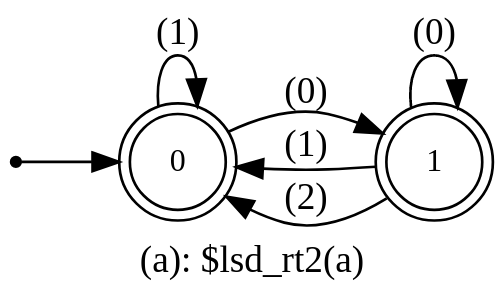
\includegraphics[width=0.4\columnwidth]{lsd_rt2.png}
    \caption{Ostrowski-$\sqrt[~]{2}$ Recognition}
    \label{fig:lsd_rt2}
\end{figure}


%%%%%%%%%%%%%%%%%%%%%%%%%%%%%%%%%%%%%
%% New Section
%%%%%%%%%%%%%%%%%%%%%%%%%%%%%%%%%%%%%
\section{The Addition Algorithm and Corresponding Automaton}


An algorithm for addition in Ostrowski numeration systems, which contains four sub-algorithms, is given in the study of Hieronymi And Terry \cite{htostrowski}. We translated each sub-algorithm into a corresponding automaton which exactly accepts the pairs $(x,y)$ where the algorithm takes in $x$ and gives result $y$.
\\The functionality of the sub-algorithms are:
\begin{itemize}
\item Algorithm 0 adds the operands.
\item Algorithm 1 checks constraint 1.
\item Algorithm 2 checks constraint 2 partially.
\item Algorithm 3 checks constraint 3 again.
\end{itemize}

\subsection{Automaton for Algorithm 0}
    \begin{definition}
    $\text{alg}_0(\alpha = [a_0; a_1,a_2,\dots])$ is a deterministic finite automaton $\{S,I,T,F\}$ over $\Sigma$ where:
    \begin{itemize}
    \item \textbf{alphabet} $\Sigma = \left\{(m,s,t) : 0\le m,s \le max(a_i),0\le t \le 2 ~max(a_i) \right\}$.
   \item it only has one state, which is also the initial and final state. $I = F = S = \left\{0\right\}$. 
   \item \textbf{transition table} :  $\left(0, \begin{pmatrix}m\\s\\t\end{pmatrix},0\right) \in T$ if $m+s=t$.
   \end{itemize}
\end{definition}

\subsection{Automaton for Algorithm 1}

    \begin{definition}
    $\text{alg}_1(\alpha = [a_0; a_1,a_2,\dots])$ is a nondeterministic finite automaton $\{S,I,T,F\}$ over $\Sigma$ where:
    \begin{itemize}
    \item \textbf{alphabet} $\Sigma = \left\{(s,t) : 0\le s \le 2 ~max(a_i),0\le t \le max(a_i) \right\}$.
   \item set of \textbf{states} $S = \left\{\left(\begin{bmatrix}a&b&c\\d&e&f\end{bmatrix},g,i\right)\right\}$. The matrix represents the input, $g$ is a carry number that is 0 or 1, and $i$ represents the position of $c$ and $f$ in the continued fraction.
   \item set of \textbf{initial states} I = $\left\{\left(\begin{bmatrix}0&0&0\\0&0&0\end{bmatrix},0,i\right)\right\}$ for all integers $i> 0$.
   \item set of \textbf{final states} F = $\left\{\left(\begin{bmatrix}a&b&c\\d&e&f\end{bmatrix},0,0\right):B(a,b,c)=(d,e,f)\right\}$ where $B$ does not change the represented values between $(a,b,c)$ and $(d,e,f)$ while the latter satisfies constraint 1.
   \item \textbf{transition table} :  $\left(\left(\begin{bmatrix}a&b&c\\d&e&f\end{bmatrix},g,i\right), \begin{pmatrix}s\\t\end{pmatrix}, \left(\begin{bmatrix}b'&c'&s'\\e&f&t\end{bmatrix},g',i-1\right)  \right) \in T$ if $(a+g,b,c,s,g)$ and $(d,b',c',s')$ represent the same value, and the latter satisfies constraint 1.
   \end{itemize}
\end{definition}

\subsection*{Automaton for Algorithm 2}

\begin{definition}
    $\text{alg}_2(\alpha = [a_1,a_2,\dots])$ is a nondeterministic finite automaton $\{S,I,T,F\}$ over $\Sigma$ where:
    \begin{itemize}
    \item \textbf{alphabet} $\Sigma = \left\{(s,t) : 0\le s,t \le max(a_i) \right\}$
   \item \textbf{set of states} $S = \left\{\left(\begin{bmatrix}a&b\\c&d\end{bmatrix},i\right)\right\}$. The matrix represents the input,  and $i$ represents the position of $b$ and $d$ in the continued fraction.
   \item \textbf{initial state} I = $\left\{\left(\begin{bmatrix}0&0\\0&0\end{bmatrix},-2\right)\right\}$.
   \item \textbf{set of final states} F = $\left\{\left(\begin{bmatrix}a&b\\c&d\end{bmatrix},i\right):a=c,b=d, i\ge0\right\}$.
   \item \textbf{transition table} :  $\left(\left(\begin{bmatrix}a&b\\c&d\end{bmatrix},i\right), \begin{pmatrix}s\\t\end{pmatrix}, \left(\begin{bmatrix}s'&a'\\t&c\end{bmatrix},i+1\right)  \right) \in T$ if the represented value of $(s,a,b)$ and $(s',a',d)$ are the same, and the $a'$ satisfies constraint 2.
   \end{itemize}
\end{definition}
\subsection*{Automaton for Algorithm 3}
\begin{definition}
    $\text{alg}_2(\alpha = [a_1,a_2,\dots])$ is a nondeterministic finite automaton $\{S,I,T,F\}$ over $\Sigma$ where:
    \begin{itemize}
    \item \textbf{alphabet} $\Sigma = \left\{(s,t) : 0\le s,t \le max(a_i) \right\}$
   \item \textbf{set of states} $S = \left\{\left(\begin{bmatrix}a&b\\c&d\end{bmatrix},i\right)\right\}$. The matrix represents the input,  and $i$ represents the position of $b$ and $d$ in the continued fraction.
   \item \textbf{initial states} I = $\left\{\left(\begin{bmatrix}0&0\\0&0\end{bmatrix},i\right)\right\}$ for all integers $i> 0$.
   \item \textbf{set of final states} F = $\left\{\left(\begin{bmatrix}a&b\\c&d\end{bmatrix},i\right):a=c,b=d, i=0\right\}$.
   \item \textbf{transition table} :  $\left(\left(\begin{bmatrix}a&b\\c&d\end{bmatrix},i\right), \begin{pmatrix}s\\t\end{pmatrix}, \left(\begin{bmatrix}b'&s'\\d&t\end{bmatrix},i-1\right)  \right) \in T$ if the represented value of $(a,b,s)$ and $(a',d,s')$ are the same, and the latter satisfies constraint 2.
   \end{itemize}
\end{definition}

Notice that since the continued fraction of a irrational number is periodic, all automatons are finite automatons, i.e. they have finite number of states.

By running the following command in Walnut, we combine our automata for these sub-algorithms, which is shown in \emph{Figure 3}:{

$$\exists y,x,w ~\text{alg}_0(a,b,w) ~\& ~\text{alg}_1(w,x) ~\& ~\text{alg}_2(x,y) ~\& ~\text{alg}_3(y,c)$$}



\begin{figure}[h]
	\centering
    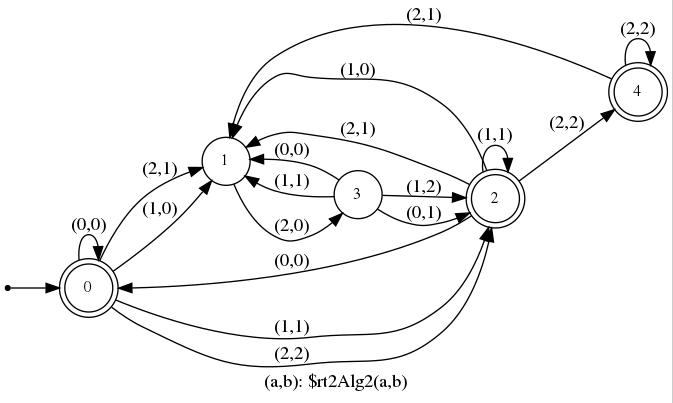
\includegraphics[width=0.6\columnwidth]{rt2Alg2_gv.jpg}
    \caption{Algorithm 2 of Ostrowski-$\sqrt[~]{2}$ (least significant digit first)}
    \label{fig:rt2_alg2}
\end{figure}
\begin{figure}[h]
	\centering
    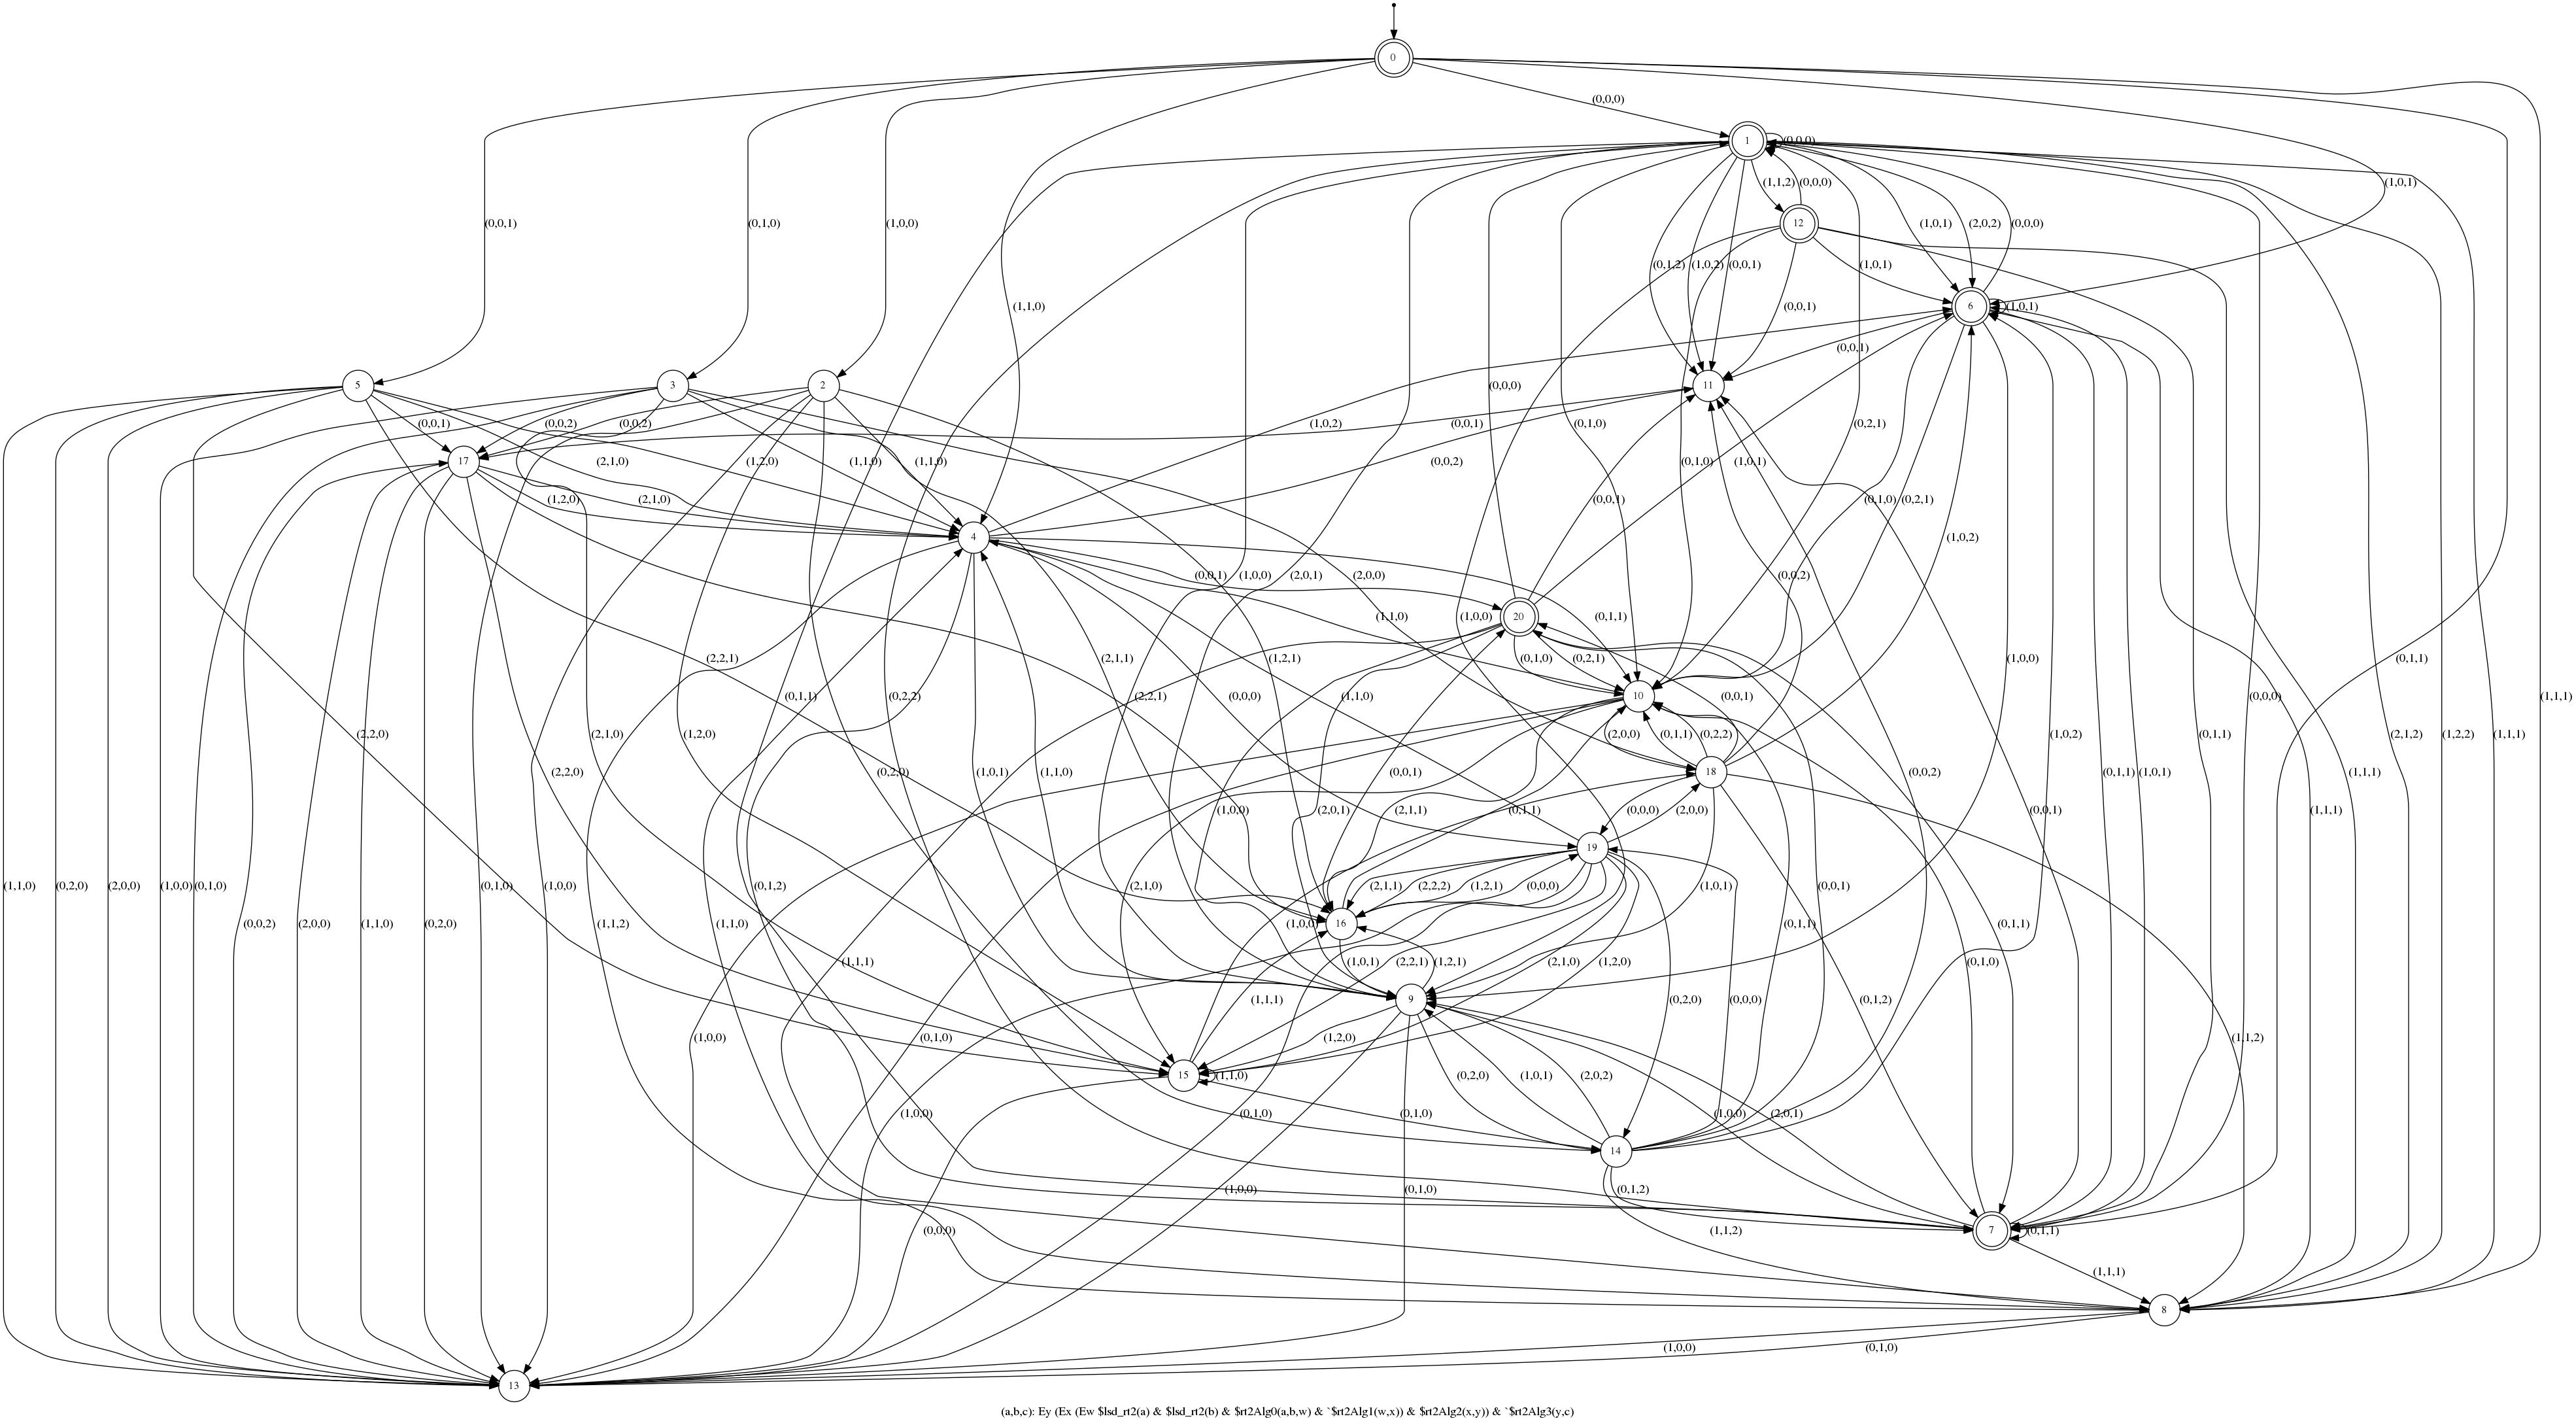
\includegraphics[width=\columnwidth]{lsd_rt2_addition_gv.jpg}
    \caption{Ostrowski-$\sqrt[~]{2}$ Addition}
    \label{fig:rt2_addition}
\end{figure}


%%%%%%%%%%%%%%%%%%%%%%%%%%%%%%%%%%%%%
%% New Section
%%%%%%%%%%%%%%%%%%%%%%%%%%%%%%%%%%%%%

\subsection{Example of addition algorithm in Ostrowski-$\sqrt{2}$}

\begin{minipage}{\columnwidth}
%Insert explanation of Algorithms 1,2 and 3, etc.

We want to add $103_{10}$ and $132_{10}$ in Ostrowski numeration with $\alpha = \sqrt[~]{2}= [1; 2,2,2,\dots].$

\begin{enumerate}
\item Convert into Ostrowski representation:\\
$109_{10} = 0\times1_{10}+0\times2_{10}+2\times5_{10}+0\times12_{10}+1\times29_{10}+1\times70_{10}= 0110200_{\sqrt[]{2}}$
\\
$138_{10} = 0\times1_{10}+0\times2_{10}+2\times5_{10}+0\times12_{10}+2\times29_{10}+1\times70_{10} = 0120200_{\sqrt[]{2}}$
\item Run Algorithm 0 (add operands): $0110200 + 0120200 \Rightarrow 0230400$.
\item Run Algorithm 1 (check constraint 1): $0230400 \Rightarrow 1020400 \Rightarrow 1021111$.
\item Run Algorithms 2 and 3 (check constraint 2): $1021111 \Rightarrow 1100111$. (Try this on \emph{Figure 2}.)
\end{enumerate}

Therefore, $0110200_{\sqrt[]{2}}+0120200_{\sqrt[]{2}}=1100111_{\sqrt[]{2}}$.

Verify:
$1100111_{\sqrt[]{2}}  = 1\times1_{10}+1\times2_{10}+1\times5_{10}+1\times70_{10}+1\times169_{10}$ = $247_{10} = 109_{10}+138_{10}$.\\

\end{minipage}

%%%%%%%%%%%%%%%%%%%%%%%%%%%%%%%%%%%%%
%% New Section
%%%%%%%%%%%%%%%%%%%%%%%%%%%%%%%%%%%%%
\section{Characteristic Sturmian word}

%include theorems, yay!
With the definition of the automaton for addition in Ostrowski numeration systems, we were able to construct similar proofs as those in Du, Mousavi, Schaeffer, and Shallit's study \cite{fibonacci} for the \textbf{characteristic Sturmian word with slope $\sqrt[~]{2}$} instead of for the original Fibonacci word.
% \vspace{0.4em}
\begin{definition}
The \textbf{characteristic Sturmian word with slope $\sqrt[~]{2}$}, which we denote as $C_2$, is the infinite word obtained as the limit of the sequence of \textbf{standard words} $s_n$ defined by{

$$ s_n=s^{d_n}_{n-1}s_{n-2} \text{ when } n\ge 2, \text{ where } s_1= 0^{d_1-1}1 \text{ and } s_0=0.$$}
\end{definition}
By having built the Ostrowski-$\sqrt[~]{2}$ numeration system and the automatic word $C_2$ in Walnut, we may use the command $C2[i]$ to return the $i^{th}$ digit of $C_2$ with the following theorem:\\

\begin{theorem}[\cite{sturmianword}, Theorem 9.1.15] Let $N\ge1$be an integer with Ostrowski$\alpha$-representation $b_jb_{j−1}\cdots b_0$. Then $C_\alpha[N] = 1$ if and only if $b_jb_{j−1}\cdots b_0$ ends with an odd number of $0$’s.
\end{theorem}


\subsection{Theorem List}

\begin{theorem} \textbf{$C_2$} \textit{contains fourth powers.}
\end{theorem}

\begin{proof}
We create the following predicate that accepts the length $n$ of fourth powers in $C_2$

$$(n > 0) \land \exists i \; \forall t<3n \;C_2[i+t] = C_2[i+n+t]$$
We then translate the predicate into one that Walnut recognizes:

$$ ? \text{msd}\_\text{rt2} ((n>0)~\&~(Ei~At (t<3 \ast n => C2[i+t] = C2[i+n+t])))$$
For this predicate, Walnut generates the following automaton:

\begin{figure}[h]
\centering
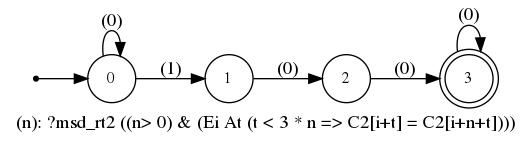
\includegraphics[width=0.7\columnwidth]{theorem5_gv.jpg}
    \caption{Automaton for the Theorem 2}
    \label{fig:Theorem}
\end{figure}
which means that there are fourth powers of length $100_{\sqrt[~]{2}},1000_{\sqrt[~]{2}},10000_{\sqrt[~]{2}},\dots$.
\end{proof}

\begin{theorem} \textbf{$C_2$} \textit{contains no fifth powers.}
\end{theorem}

\begin{proof}
We create the following predicate that accepts the length $n$ of fifth powers in $C_2$

$$(n > 0) \land \exists i \; \forall t<4n \;C_2[i+t] = C_2[i+n+t]$$
We then translate the predicate into one that Walnut recognizes:

$$ ? \text{msd}\_\text{rt2} ((n>0)~\&~(Ei~At (t<4 \ast n => C2[i+t] = C2[i+n+t])))$$
For this predicate, Walnut generates the following automaton:

\begin{figure}[h]
\centering
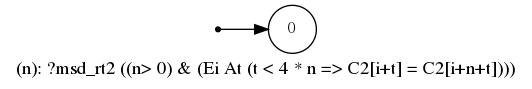
\includegraphics[width=0.7\columnwidth]{theorem5_1_gv.jpg}
    \caption{Automaton for the Theorem 3}
    \label{fig:Theorem}
\end{figure}
which means that there are no fifth powers.
\end{proof}

\begin{theorem}  All antisquare factors of \textbf{$C_2$} can only be: 01, 10, 1001, 101010, 010101, and 10100101.
\end{theorem}

\begin{proof}
Walnut outputs the following automaton that accepts the period $n$ of the antisquares in $C_2$:

\begin{figure}[h]
\centering
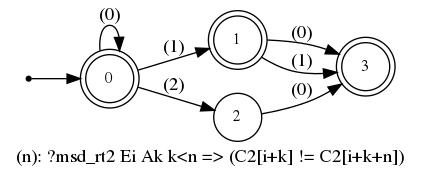
\includegraphics[width=0.7\columnwidth]{theorem11_gv.jpg}
    \caption{Automaton for the Theorem 4} 
    \label{fig:Theorem}
\end{figure}
which means that all antisquares in $C_2$ have period 1,2,3,4. Therefore, antisquare factors of $C_2$ can only be: 01, 10, 1001, 101010, 010101, and 10100101.

Note: All mentioned antisquares are indeed factors of $C_2$.
\end{proof}

\begin{theorem} \textbf{$C_2$} \textit{has palindromes of any length.}
\end{theorem}

\begin{proof}
Walnut generates the following automaton for that accepts the length of palindromes in $C_2$:

\begin{figure}[h]
\centering
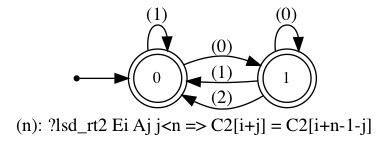
\includegraphics[width=0.5\columnwidth]{theorem12_gv_copy.jpg}
	\vspace*{-5mm}
    \caption{Automaton for the Theorem 5} 
    \label{fig:Theorem}
\end{figure}

which means that there palindromes of any length in $C_2$.
\end{proof}
\newpage
\begin{theorem} \textbf{$C_2$} \textit{is linearly recurrent.}
\end{theorem}

\begin{proof}
We create the following Walnut predicate that accepts if $C_2$ is linearly recurrent:
$$?msd_{rt2} ~An,i,j ~Es ~(j<=s ~\& ~s<=j+4\ast ~n) ~\& ~(Ap ~p<n ~=> ~(C2[s+p] ~= ~C2[i+p]))":$$
For this predicate, Walnut generates the following automaton:

\begin{figure}[h]
\centering
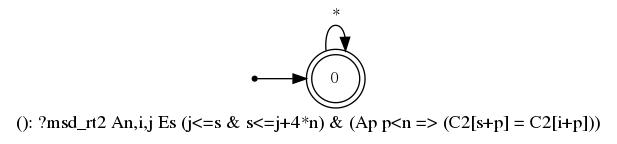
\includegraphics[width=0.7\columnwidth]{theorem23_6_gv.jpg}
    \caption{Automaton for the Theorem 6}
    \label{fig:Theorem}
\end{figure}

which means accepts. Therefore, $C_2$ is linearly recurrent.
\end{proof}
%Maybe a future work section here?
\section{Future Work}
\begin{itemize}
\item Use the automata for Ostrowski numeration systems to prove more theorems regarding characteristic Sturmian words.
\item Investigate the critical exponent of infinite balanced words.
\item Find a faster algorithm to generate automata for Ostrowski addition.
\item Provide a general automaton for Ostrowski numeration, which would include $\alpha$ as input.
\end{itemize}


\begin{thebibliography}{9}
\bibitem{walnut} 
Mousavi, H. (2016). \textit{Automatic theorem proving in Walnut}. arXiv preprint arXiv:1603.06017.
 
\bibitem{htostrowski} 
Hieronymi, P., and Terry Jr, A. (2018). \textit{Ostrowski Numeration Systems, Addition, and Finite Automata}. Notre Dame Journal of Formal Logic, 59(2), 215-232.
 
\bibitem{fibonacci} 
Du, C. F., Mousavi, H., Schaeffer, L., and Shallit, J. (2014). \textit{Decision algorithms for Fibonacci-automatic words, with applications to pattern avoidance}. arXiv preprint arXiv:1406.0670.

\bibitem{sturmianword}
J.-P. Allouche and J. Shallit, \textit{Automatic Sequences}, Cambridge 2003.

\end{thebibliography}
\end{document}